\newcommand{\pd}[2]{\displaystyle\frac{\displaystyle\partial #1}{\displaystyle\partial #2}}
\newcommand{\vol}[1]{\langle #1 \rangle}
\newcommand{\sigy}{\sigma_{\rm y}}
\newcommand{\epse}{\varepsilon^{\rm e}}
\newcommand{\epsp}{\varepsilon^{\rm p}}

\newcommand{\epst}{\varepsilon}
\newcommand{\sig}{\sigma}
\newcommand{\Fp}{f^{\rm p}}
\newcommand{\Fd}{f^{\rm d}}
\newcommand{\norm}[1]{| #1 |}

\section{Motivation}

\frame{\frametitle{Fatigue damage}

\uncover<1->{
		\twocol{	\begin{itemize}
				\item Cyclic loading
			\end{itemize}
			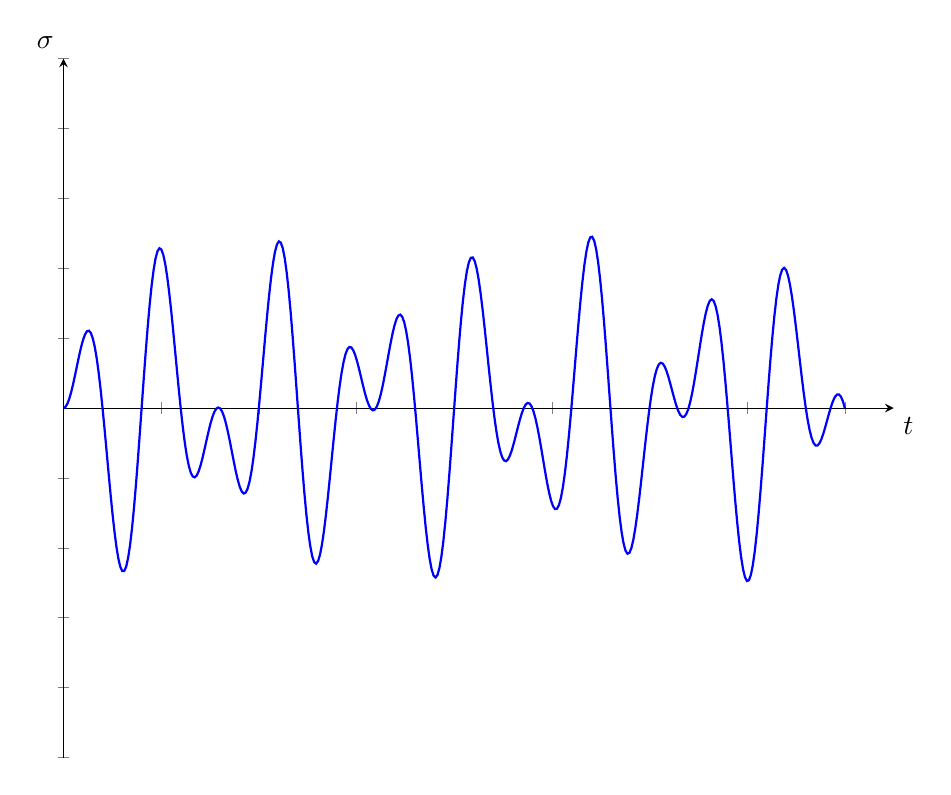
\begin{tikzpicture}[scale=1]
			\begin{axis}[axis x line=center, axis y line=center,
			xticklabels={},yticklabels={},xlabel style={below right},
			ylabel style={above left},ymin=-1,ymax=1,xmin=0,xmax=8.5,
			width=\textwidth,xlabel=$t$,ylabel=$\sigma$]
			\addplot [color=blue,thick,mark=none,domain=0:8,samples=400]{sin(2*\x r)*0.5*sin(pi / 2 * 5 * \x r)} ;
			\end{axis}
			\end{tikzpicture}
		}{
			\centering
			\uncover<2->{\hfil
				\begin{itemize}
					\item Damage
				\end{itemize}
				
					\only<2>{\includegraphics[width=0.9\textwidth]{./img/Windturbine.jpg}\\[-0.3cm]}

					\only<3->{\includegraphics[width=0.9\textwidth]{./img/bridge.jpg}\\[-0.3cm]}
					\uncover<2-3>{\vspace*{0.1cm} {\tiny Image by alegri / 4freephotos.com}}
					\uncover<4>{	
						
						\begin{tikzpicture}[x=1cm,y=1cm,overlay]
							\node at (1.7,0.6) {
								\begin{tikzpicture}[x=1cm,y=1cm,overlay]
								\node [draw,fill,circle,radius=1pt,inner sep=0.5pt] at (-0.7,1.5) {};
							\draw (-2,-0.3) -- (-0.7,1.5);
							\draw (-0.5,-0.3) -- (-0.7,1.5);
							\draw (-2,-1.8) -- (-0.7,1.5);
							\draw (-0.5,-1.8) -- (-0.7,1.5);
						\end{tikzpicture}	};
							\node at (0.45,-0.45) {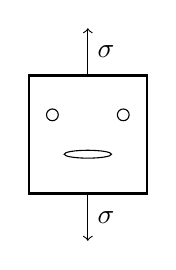
\begin{tikzpicture}[x=1cm,y=1cm,rotate=-90]
								\draw [thick,fill=white] (-2,-1.8) rectangle ++(1.5,1.5);
								\node [draw,circle,radius=1pt,inner sep=1.5pt] at(-1.5,-1.5) {};
								\draw (-1,-1.05) ellipse (0.5mm and 3mm);
								\node [draw,circle,radius=1pt,inner sep=1.5pt] at(-1.5,-0.6) {};
								\draw [->,thin] (-.5,-1.05) -- ++(0.6,0) node [right,pos=0.5] {$\sigma$};
								\draw [->,thin] (-2,-1.05) -- ++(-0.6,0) node [right,pos=0.5] {$\sigma$};
								\end{tikzpicture}};
						\end{tikzpicture}
						}
				}
				
				}
			}
			{
			
			}
	}





\frame{\frametitle{Fatigue damage}
	
		\twocol{	\begin{itemize}
				\item LATIN method\\[0.5cm]
				%		\scriptsize
				{\footnotesize $\bullet$ An approximation on the \textbf{whole time-space domain} is obtained.} \\	
				{\footnotesize $\bullet$ The balance equation is solved as a \textbf{linear} problem.} 
			\end{itemize}
		}{
			\centering
			\uncover<1->{\hfil
				\uncover<1->{	\begin{itemize}
						{\item Model order reduction (MOR)\\[0.7cm]}
					{\footnotesize $\bullet$ Proper generalised decomposition (PGD)\\ \tiny [Chinesta, Ladev{\`e}ze 2014] }
	%	[Ladeveze 1985,1999; Chinesta, Ladev{\`e}ze 2014]}\\
	$\hfil \epsp(x,t) \approx \sum_{i=1}^{n} \bar{\varepsilon}^{\rm p}_i(x) \ \lambda_i(t)$
					\end{itemize}}	
				}
			}
			{
			
			}
		}



\section{Numerical example}

\frame{\frametitle{Numerical example}
		\vspace*{-0.5cm}
	\begin{center}
		\hspace{1cm}
		\begin{tikzpicture}[x=1cm,y=1cm,scale=0.5]
		\fill [ultra thick] (0,-0.05+1.75) rectangle (4,0.05+1.75) node [above,pos=0.5] {};
		\fill [ultra thick] (0,-0.05+1.25) rectangle (4,0.05+1.25) node [above,pos=0.5] {};
		\fill [thick] (4,-0.05+1.25) rectangle (4.05,0.05+1.75) node [above,pos=0.5] {};
		
		\draw [->,thin] (4,0+1.5) -- (4.5,0+1.5) node [below right,pos=0.5] {$\bar{u}$};
		\draw [ultra thick] (0,-0.5+1.5) -- (0,0.5+1.5);
		\path [pattern=north west lines] (-0.25,-0.5+1.5) rectangle (0,0.5+1.5);
		\begin{axis}[at={(0.8\textwidth,-2)},axis x line=center, axis y line=center,
		xticklabels={},yticklabels={},xlabel style={below right},
		ylabel style={above left},ymin=-1,ymax=1,xmin=0,xmax=8.5,
		width=0.5\textwidth,xlabel=$t$,ylabel=$\bar{u}$]
		\addplot [color=blue,thick,mark=none,domain=0:8,samples=400]{0.5*sin(pi / 2 * 5 * \x r)} ;
		\end{axis}
		\end{tikzpicture}\\
		%	{ \tiny Uniaxial visco-plastic bar with cyclic loading without considering dynamic effects}\\[0.5cm]

	\vspace*{-0.3cm}
%	\hspace*{-0.5cm}
		\includegraphics[width=0.7\textwidth,clip]{img/030_2}\\
		\end{center}
	%		\centering {\scriptsize Damage evolution at convergence}}{}
%	\input{img/sh_bar}
}

\frame{
	\frametitle{Damage evolution}
\centering
	\includegraphics[width=4cm,clip]{img/cube2.png} \hfil
	\includegraphics[width=4.3cm,clip]{img/cube}\\
	\hspace*{0.3cm}
	\includegraphics[width=4cm,clip]{img/hole.png} \hfil 
	\includegraphics[width=5cm,clip]{img/hole2}
	%		\centering {\scriptsize Damage evolution at convergence}}{}
}


\frame{\frametitle{Variable loading}
	\small
	Different types of loads are applied on different structures
	\begin{itemize}
		\item  Pressure vessels
		\item Bridges
		\item Aircraft 
	\end{itemize}
	These loads may be characterised in two different groups
	\begin{itemize}
		\item Deterministic loads, e.g. loads on a pressure vessel.
		\item Stochastic loads, e.g. wind and ocean forces.\\
		A description of such loads can only be given using a statistical approach.
	\end{itemize}
	
	
	\begin{block}{ \centering Description of load histories.}
\end{block}}


\frame{
	\frametitle{Block loading}
	\small
	\begin{itemize}
		\item Cycle counting methods.
		\item Randomness may be introduced in the order of the blocks.
		{\begin{center}
				\includegraphics[width=0.6\textwidth,clip]{img/blockloading.eps}
		\end{center}}
		\item Miner's rule: $ D=r=\sum_{i=1}^{k} \frac{n_i}{{N_f}_i}$\\
		\uncover<2->{
			\centering
%				\includegraphics[width=0.33\textwidth,clip]{img/miner.eps} 
				\includegraphics[width=0.33\textwidth,clip]{img/blockloading_D.eps}}
	\end{itemize}
}


\frame{
	\frametitle{Standardised load histories}
		\footnotesize 
	\begin{itemize}
		\item Loadings are reported in an exceedance diagram (spectrum shape).
		\item The root mean square for each block is sometimes defined.
	\end{itemize}
\centering
\begin{minipage}{0.4\textwidth}
\centering
\includegraphics[width=1\textwidth,clip]{img/exceedence}\\[0.1cm]
\centering
\tiny 
\begin{tabular}{|c|c|}
	\hline 
	Amplitude & \# half cycles \\ \hline
	60 & 1 \\ \hline
	50 & 2 \\ \hline
	40 & 3 \\ \hline
	30 & 10\\ \hline
	20 & 20\\	\hline 
\end{tabular}
\end{minipage}\hfil\begin{minipage}{0.4\textwidth}
\centering
\includegraphics[width=\textwidth,clip]{img/exceedence2}
\end{minipage}
}
\frame{
	\frametitle{Random loading}
	\footnotesize 
	\begin{itemize}
		\item defined by a power spectral density function (PSD).
		\item Variable amplitudes and frequencies.
	\end{itemize}
\begin{minipage}{0.4\textwidth}
	\centering
\includegraphics[width=1.3\textwidth,clip]{img/psd}
\end{minipage}\hspace*{1cm}\begin{minipage}{0.4\textwidth}
\begin{equation*}
\begin{split}
a_i &= \sqrt{2 \int_{\omega_1}^{\omega_2}\ S(\omega) \ \rm{d} \omega} \\[0.5cm]
&\approx \sqrt{2 \ S_i(\omega_i) \ \Delta \omega_i} \\[0.5cm]
\eta &= \sum_{i=1}^{n} a_i \ \cos(\omega_i \ t + \varphi_i )
\end{split}
\end{equation*}
\end{minipage}

}


\frame{
	\frametitle{Outlook}
	\footnotesize 
	\begin{itemize}
		\item 3D continuum damage model.
		\item LATIN-PGD framework.
		\item Literature review on variable loading.
	\end{itemize}
	{\color{luhBlue} Future activities:}
	\begin{itemize}
		\item Two-time scale approach
			\begin{itemize}
			\item Introducing block loading.
			\item Accounting for standardised load histories. 
			\end{itemize}
		\item HCF computations.	
		\item Dynamic effects.
	\end{itemize}
	\centering
	\uncover<2>{
	\begin{block}{ \centering Thank you for your attention.}
	\end{block}}
}
